\section{Implementierung}
\label{sec: implementation}
In dieser Sektion wird sich ausgiebig mit der Implementierung der zuvor festgelegten Anforderungen auseinandergesetzt.

\subsection{Server}
\label{sec: server}
Da zu diesem Zeitpunkt bereits Librarys zur Authentifizierung existieren, wurde sich zuerst mit der Library Devise auseinandergesetzt.

\subsubsection{Devise}
\label{sec: devise}
Devise ist eine Ruby on Rails Library mit der sich eine flexible Authentifizierung ermöglichen lässt. Es bietet ein vorgefertigtes Datenbankschema für registrierte Benutzer, einen leichten Umgang mit OmniAuth und Funktionen wie beispielsweise das Senden einer E-Mail bei Registrierung. Im Datenbankschema enthalten ist ein Log-System mit dem beispielweise der Zeitpunkt der letzten Anmeldung eines Benutzers festgehalten werden kann. \todo{Warum nicht genommen? Was für Probleme traten auf?}

\subsubsection{Anmeldung eines Benutzers}
\label{sec: sign-in-imp}
Die Anmeldung mittels oAuth2 oder Passwort wurde mit Omniauth ermöglicht. Hierbei wurde zuerst Omniauth selber dem derzeitigen Projekt hinzugefügt und darauffolgend die Gems zur Authentifizierung mittels Google, GitHub und Passwort. Um die einzelnen Provider nutzen zu können müssen diese in einem initializer (Listing \ref{lst:added_providers}) deklariert werden. Ein initializer wird nach dem Rails Framework und den dazugehörigen Gems geladen. Bei der Deklarierung der Provider ist zu beachten, dass Provider wie Google oder GitHub eine jeweilige ID und einen Secret-Key als Parameter benötigen. Diese werden jeweils auf den offiziellen Seiten der Provider erstellt. Dabei musste darauf geachtet werden, dass diese ID und dieser Secret-key über eine Umgebungsvariable mit in das Projekt eingebunden wird. Umgebungsvariablen werden in dem Fall in der Kommandozeile vor das Kommando zum starten des Projektes gesetzt. Nach dem das Kommando zum starten des Servers ausgeführt wurde, kann auf die Werte der zuvor festgelegten Umgebungsvariablen zugegriffen werden. Die Verwendung von Umgebungsvariablen ist besonders bei Blattwerkzeug vonnöten, da es sich um ein quelloffenes Projekt handelt und jeder den bereits produzierten Code einsehen kann.

    \todo[inline]{Letzter Schritt: Secrets sind Passwörter und deswegen geheim und nicht im Repo. Das ist übrigens nicht nur ein Problem bei OpenSource-Projekten. Auch Spotifiy hält den Facebook-OAuth-Schlüssel vor 99.99\% der Mitarbeiter geheim}

    \lstinputlisting[language=Ruby, style=CodeView, caption=Zu Omniauth hinzugefügte Provider, captionpos=b, label={lst:added_providers}]{snippets/omniauth-initializer.rb}

    \todo[inline]{Zeile 5 \& 6 des Listings inkonsistent bei Schreibweise}

Bei der Erstellung des User und des Identity Models wurde sich zuerst damit beschäftigt\todo{ugs, es wurde diskutiert, abgewogen, entschieden, ...} welche Attribute die jeweiligen Models haben sollen. Hierbei steht das Identity Model für alle hinzugefügten Authentifikations-Möglichkeiten eines Benutzers. Dabei wurde darauf geachtet, welche Attribute später dem Client zur Verfügung gestellt werden sollten und welche für spätere Controller Funktionen benötigt werden.

\begin{figure}[h]
	\includegraphics[width=\textwidth]{graphics/identities_table.png}
	\caption{identities Tabelle}
	\label{fig:identities_table}
\end{figure}

\todo[inline]{Beschreibung der Spalten nach Tabelle trennen}


\begin{description}
	\item[uid (Abbildung \ref{fig:identities_table})]\hfill\\
	Die uid ist ein String der zur eindeutigen Identifikation des Kontos eines Providers dient. Dabei kann die uid beispielsweise eine Zahl oder eine E-Mail sein. Mit der uid wird festgestellt ob ein bestimmtes Konto bereits mit einem Benutzer verknüpft ist.
	\item[provider (Abbildung \ref{fig:identities_table})]\hfill\\
	Das provider Attribut wird mit dem jeweiligen Provider-Namen beschrieben. Dabei sind die Namen wie in Listing \ref{lst: added_providers} definiert. Da die Namen jedoch von den installierten Gems stammen\todo{definiert werden} ist eine Änderung dieser Namen nicht ohne weiteres Möglich.
	\item[provider\_data (Abbildung \ref{fig:users_table})]\hfill\\
	Das provider\_data Attribut wird mit jeglichen Daten beschrieben, die ein Provider über den authentifizierten Benutzer zurückliefert.\todo{Konkrete Beispiele für Google und Github}
	\item[own\_data (Abbildung \ref{fig:identities_table})]\hfill\\
	Das own\_data Attribut wird mit den Daten beschrieben die Blattwerkzeug für den Benutzer vorgesehen hat. Dies kann beispielsweise der Token zur Aktivierung einer E-Mail sein.
	\item[type (Abbildung \ref{fig:identities_table})]\hfill\\
	Das type Attribut wird, sobald es der Tabelle hinzugefügt wurde, von Rails automatisch interpretiert. Hierbei handelt es sich um \gls{STI}. \gls{STI} ist eine Möglichkeit Objekt-Orientierung in einer Relationellen Datenbank zu emulieren. Dabei ist die Tabelle identities und dessen Model (Identity) die Basisklasse und die in type festgelegten Klassen, die Abgeleiteten. Das type Attribut ermöglicht einen sofortigen Zugriff auf die Klasse des Providers einer ausgewählten Identity.
\end{description}

\begin{figure}[h]
	\includegraphics[width=\textwidth]{graphics/users_table.png}
	\caption{users Tabelle}
	\label{fig:users_table}
\end{figure}

\begin{description}
	\item[display\_name (Abbildung \ref{fig:users_table})]\hfill\\
	Das display\_name Attribut steht für den Anzeigenamen des Benutzers. Dieser ist jedoch nicht einzigartig und lässt sich beliebig oft verändern. Das hat zur Folge, dass mehrere Benutzer denselben Anzeigenamen haben können.
	\item[email (Abbildung \ref{fig:users_table})]\hfill\\
	Das email Attribut steht für die primäre E-Mail eines Benutzers. Die primäre E-Mail wird verwendet sobald eine E-Mail von Blattwerkzeug an den Benutzer gesendet werden soll. Dies ist wichtig, da jedes verknüpfte Konto eine unterschiedliche E-Mail besitzen darf. Die primäre E-Mail wird bei Erstellung eines Benutzers gesetzt, außer ein Benutzer authentifiziert sich über einen Provider dessen Rückgabe keine E-Mail enthält.
\end{description}

\todo[inline]{Überschrift}
\begin{description}
	\item[Anmeldung mittels \gls{oAuth2}]\hfill\\
	Bei einer Anmeldung mittels \gls{oAuth2} wurde bei dem Provider über den sich authentifiziert wird, eine Redirect Url hinterlegt. Auf diese wird der jeweilige Benutzer nach Authentifikation zurückgeleitet. Die Route zu der Redirect Url zeigt auf die Funktion mit dem Namen \enquote{Callback} im \enquote{AuthController}. Die Callback Funktion prüft auf das vorhanden sein der vom Provider zurückgelieferten Daten. Sollte bisher keine Identität mit den Daten des Providers erstellt worden sein wird eine neue Identität angelegt. Sollte ein angemeldeter Benutzer diese Funktion ausführen wird ihm eine neue Identität zu seinem Benutzer hinzugefügt. Sollte es sich um keinen angemeldeten Benutzer handeln, wird zusätzlich ein neuer Benutzer erstellt. Da jeder Provider unterschiedliche Daten zurückliefert wird beim anlegen einer neuen Identität zwischen den einzelnen Providern unterschieden. Jeder Provider besitzt eine Abgeleiteteklasse der Basisklasse Identity und greift innerhalb seiner Klasse auf die für ihn relevanten Daten zu. Sollte eine Identität mit den zuürckgelieferten Daten bereits existieren, wird ohne Erstellung einer Identität fortgefahren. Mit der erstellten oder existierenden Identität werden die Benutzerinformationen in die Payload eines \gls{JWT} geschrieben. Bei den Benutzerinformationen handelt es sich um die id, den display\_name und die Rollen eines Benutzers. Die Funktionen zu Erstellung eines \gls{JWT} wurden hierbei in einen Helper ausgelagert und die Gültigkeitsdauer des erstellten \gls{JWT} beläuft sich auf eine Stunde.

	\todo[inline]{Diagramm hilft}

      \item[Anmeldung mittels Passwort]\hfill\\
      \todo[inline]{Visualisierung als Automat (Zustände / Übergänge) zur Veranschaulichung des Prozesses vermutlich hilfreich}
      \todo[inline]{Allgemein: Mehr Struktur, in diesem Punkt verstecken sich zuviele eigenständige Funktionen}
      Die Anmeldung mittels Passwort wurde mittels Omniauth Identity\todo{Link / Quelle} ermöglicht. Omniauth Identity ist ebenfalls eine Strategie mit der die Möglichkeit gegeben ist, sich über ein Passwort bei Blattwerkzeug anzumelden. Ebenso wie die Developer Strategie, bietet auch diese Strategie die Möglichkeit ein vorgefertigtes Formular für Anmeldung und Registrierung zu erstellen. Jedoch ist es bei dieser Strategie optional und eine ausschließliche Kommunikation über ein API ist möglich.

	Bei dem Nutzen dieser Strategie fiel auf, dass die Daten übermittelt wurden sie jedoch nicht richtig verarbeitet werden konnten (Listing \ref{lst:register_omniauth_identity}). Das hatte zur Folge, dass mit der Erstellung eines Models, welches mit als Parameter im iniziliazer angegeben werden kann, nicht ordnungsgemäß fortgefahren werden konnte. Um fortzufahren wäre es möglich eine eigene Strategie für Omniauth zu entwickeln oder auf die von Omniauth Identity mitgelieferten Optionen zurück zugreiffen.

	 \lstinputlisting[language=Ruby, style=CodeView, caption=Aufgerufene Funktion bei POST Request (Omniauth Identity), captionpos=b, label={lst:register_omniauth_identity}]{snippets/omniauth-identity-registration.rb}

	Omniauth Identity bietet die Möglichkeit bei Registrierung auf eine Funktion zu verweisen. Diese Funktion muss ebenfalls im iniziliazer\todo{typo} angegeben werden. (Listing \ref{lst:added_providers}). Sollte bei der Erstellung des Models ein Fehler auftreten (Listing \ref{lst:register_omniauth_identity}), wird die Funktion im zuvor festgelegten iniziliazer aufgerufen. Letztendlich wurde sich in der Thesis für diese Methode entschieden. Hierbei wurden jegliche Funktionen innerhalb des AuthControllers und außerhalb der Strategie genutzt. Dieses Verhalten der Strategie, entspricht jedoch nicht dem Schema Omniauths (Sektion \ref{sec:omniauth}). Diese Tatsache wurde jedoch erst im späten Verlauf der Thesis eindeutig.

	Bevor eine Anmeldung mittels Passwort stattfinden kann, wurde eine Registrierungs-Möglichkeit hinzugefügt. Die \enquote{register} Funktion arbeitet ähnlich wie die callback Funktion\todo{welche}. Der Unterschied besteht darin, dass die register Funktion einen simulierten Hash in der Struktur Omniauths erhält und mit diesem versucht eine neue Identität zu erstellen. Beim erstellen einer neuen Password-Identität wird ein Verifizierungs-Token generiert. Dieser Verifizierungs-Token ist eine \gls{UUID} und wird zur Verzifizierung der Identität genutzt. Nachdem eine Identität erstellt wurde, sendet der Server mithilfe der Basisklasse ActionMailer eine Bestätigungsmail. Diese Bestätigungsmail verhindert das Registrieren von willkürlichen E-Mail Adressen. Außerdem wird  mit der Bestätigungsmail eine E-Mail Adresse auf ihre existens geprüft. Die Bestätigungsmail besteht aus einem Hyperlink zu einer \gls{URL} Blattwerkzeugs in der, der Verifizierungs-Token enthalten ist. Sobald dieser \gls{URL} besucht wird, wird die Indentität als bestätigt gekennzeichnet. Dies erfolgt durch das Setzen des confirmed Feldes im JSON Blob Attribut own\_data.

	Da es vorkommen kann, dass eine Verifizierungsmail nicht an der angegebene E-Mail ankommt, wurde hierfür eine Funktion im IdentitiesController geschrieben. Diese Funktion prüft die übermittelte E-Mail auf ihre existens in der Blattwerkzeug-Datenbank und ob diese bereits verifiziert wurde. Sollte diese E-Mail nicht verifiziert sein wird eine neue Verifizierungsmail versendet. Gleichzeitig wird jedoch auch eine Wartezeit von zwei Minuten im own\_data Attribut festgelegt. Die Wartezeit zum versenden einer neuen Verifizierungsmail soll verhindern, dass eine E-Mail Adresse mit Verifizierungsmails überhäuft werden kann.

	Sollte eine Identität mit einem Passwort bereits vorhanden sein, kann sich mit seiner E-Mail und seinem Passwort angemeldet werden. Bei der Anmeldung wird das Passwort zur angegebenen E-Mail überprüft. Zusätzlich wird geprüft ob die E-Mail verifiziert wurde. Sollten diese Sicherheitsabfragen erfolgreich durchlaufen sein wird wie bei der Anmeldung mittels \gls{oAuth2} ein \gls{JWT} ausgestellt in dem die Benutzerinformationen gespeichert werden.

	Da im Laufe der Zeit die Möglichkeit besteht, dass Benutzer ihr Passwort vergessen haben, wurde hierfür eine Funktion im IdentitiesController erstellt. Damit ein Passwort zurück gesetzt werden kann muss die übermittelte E-Mail Adresse als Passwort Identität vorhanden sein. Sollte diese Identität vorhanden sein, wird ein password\_reset\_token erstellt. Dieser password\_reset\_token ist eine \gls{UUID} und wird im own\_data JSON Blob Attribut gespeichert. Ebenfalls zum own\_data Attribut hinzugefügt wird ein Feld password\_reset\_token\_exp. Dessen Wert beläuft sich auf die aktuelle Uhrzeit plus dreißig Minuten. Nachdem die festgelegte Uhrzeit des password\_reset\_token\_exp Feldes überschritten wurde, kann der Zurücksetzungs-Token nicht mehr verwendet werden. Damit das Passwort trozdessen zurückgesetzt werden kann, muss ein neuer Zurücksetzungs-Token angefordert werden. Die Ablaufzeit eines Zurücksetzungs-Tokens hat den Vorteil, dass sollte beispielsweise ein Angreiffer Zugriff auf den Browserverlauf haben, dieser nicht die Möglichkeit erhält das Passwort dieses Benutzers zu verändern. Die E-Mail die beim Kennwort zurücksetzen versendet wird, wird an die primäre E-Mail verschickt und enhält einen Hyperlink zum wiederherstellen des Passwortes. Der Hyperlink beinhaltet den password\_reset\_token und nachdem ein neues Passwort ausgewählt wurde, wird von jeder Passwort-Identität des Benutzers das Passwort geändert.
\end{description}

\subsubsection{Autorisierung}
\label{sec:server-authorisation}
Sobald ein Benutzer angemeldet ist, wird bei jedem Request ein \gls{JWT} mit an den Server gesendet. Dieser wird Serverseitig auf seine Gültigkeit geprüft. Hierbei prüft der Server ob dieser \gls{JWT} seine Ablaufzeit nicht überschritten hat und ob der \gls{JWT} die Signatur des Servers beinhaltet. Diese Überprüfung authentifiziert einen Besucher als angemeldeten Benutzer und wird von der Library jwt\todo{Quelle} übernommen.

Damit zwischen den Benutzern unterschieden werden kann, wurden drei Globale-Rollen eingebaut.

\todo[inline]{Unklar: Was genau wurde extra \enquote{eingebaut}? Ich halte das eher für eine Konvention. Und zwischen Benitzern unterscheidet man anhand ihrer ID ;-) Ich weiß was gemeint ist, aber geh hier nochmal in dich und formulier sauber aus inwiefern diese (sinnvolle!) Konvention dir hilft.}

\begin{description}
	\item[guest]\hfill\\
	Die guest Rolle wird einem einzigen Benutzer zugewiesen. Dieser Benutzer beschreibt einen unangemeldeten Besucher. Jedem der Blattwerkzeug besucht und sich nicht anmeldet wird dieser Gast-Benutzer zugewiesen. Der Gast-Benutzer besitzt keine Möglichkeit Änderungen, die über Bedienelemente ermöglicht werden, zu speichern oder zu löschen.
	\item[user]\hfill\\
	Die user Rolle stellt einen angemeldeten Benutzer dar. Sollte bei einer Identitäts Erstellung festgestellt werden, dass der aktuelle Benutzer keine Globale-Rolle admin oder user besitzt, wird automatisch die user Rolle hinzugefügt. Mit der user Rolle wird das Erstellen, Speichern und Löschen von Projekten ermöglicht. Dies bezieht sich jedoch nur auf eigene Projekte.
	\item[admin]\hfill\\
	Die admin Rolle stellt einen administrierenden Benutzer dar. Jegliche Operationen die mit der user Rolle ausgeführt werden können, können ebenfalls mit der admin Rolle ausgeführt werden. Darüberhinaus kann ein Benutzer mit der admin Rolle, jegliche Projekte bearbeiten und beschränkt sich nicht auf seine eigenen. Der Admin-Benutzer besitzt zusätzliche Funktionen mit denen er beispielsweise eine Neuigkeit, die Clientseitig auf der Startseite angezeigt wird, erstellen kann.
\end{description}

Um den Zugriff auf das Verwalten eines Projektes oder einer News zu beschränken, wurde jeweils eine Policy (Listing \ref{lst:project_policy}) angelegt. Bei der Erstellung einer Policy fiel auf, dass es sinnvoller ist den Ersteller einer News oder eines Projektes in der jeweiligen Tabelle mit zu hinterlegen. Dafür wurde ein neues Attribut owner der projects und news Tabelle hinzugefügt. Dieses owner Attribut ist ein Fremdschlüssel und bezieht sicht auf die users Tabelle. Die Beziehung die folgedessen enstand ist eine 1:n. Das beudetet ein Benutzer kann beispielsweise verschiedene Projekte besitzen, jedoch ein Projekt nur einen Benutzer haben. Den Vorteil den das hinzufügen des owner Attributes hat, ist der direkte Zugriff auf die erstellten Projekte eines Benutzers. Außerdem kann zwischen einem Ersteller eines Projektes und einem Benutzer der eine Rolle zum bearbeiten eines Projektes erhalten hat, unterschieden werden kann.

\lstinputlisting[language=Ruby, style=CodeView, caption=Policy zur Autorisierung eines Zugriffs auf ein Projekt, captionpos=b, label={lst:project_policy}]{snippets/project_policy.rb}

Da Blattwerkzeug bereits eine Passwortabfrage eingebaut hatte (Listing \ref{lst:controller_function_before}) dessen Anmeldedaten sich auf user und user beschränkten, mussten diese durch die von Pundit mitgelieferte authorize (Listing \ref{lst:controller_function_after}) Methode ersetzt werden.

\lstinputlisting[caption=Controller-Funktion ohne Integrierung Pundits, style=CodeView, captionpos=b, label={lst:controller_function_before}]{snippets/controller_authorisation_before.rb}

\begin{minipage}{\linewidth}
	\lstinputlisting[caption=Controller-Funktion mit Integrierung Pundits, style=CodeView, captionpos=b, label={lst:controller_function_after}]{snippets/controller_authorisation_after.rb}
\end{minipage}
\todo[inline]{Ruby syntax highlighting fehlt 2x}
\todo[inline]{Warum mal minipage und mal nicht?}

\todo[inline]{\enquote{may\_perform} sollte ein eigener Punkt mit Überschrift sein}
\begin{description}
	\item[may\_perform]\hfill\\
	Sobald sich mit den Rollen beschäftigt wurde, stellte sich die Frage wie die Bedienelemente in Abhängigkeit von den Rollen Clientseitig angezeigt werden sollten. Hierbei gab es die Möglichkeit ein eigenes Pundit (Sektion \ref{sec: pundit}) ähnliches Mustur zu implementieren oder den Server bei jedem Bedienelement zu fragen, ob der aktuelle Benutzer Zugriff auf das Bedienelement hat. In der Thesis wurde sich für den zweiten Weg entschieden, da bei einer zusätzlichen Clientseitigen Überprüfung, Client und Server gepflegt werden müssten. Sollte es vorkommen, dass die Pflege des Serverseitigen-Teils vergessen wurde, stellt dieses ein Sicherheitsrisiko dar. Clientseitige Anwendungen werden auf dem Entgerät eines Benutzers ausgeführt. Folgedessen besteht die Möglichkeit die Anwendung zu manipulieren.

	Die Serverseitige Überprüfung der Bedienelemente wurde mittels der may\_perform Funktion realisiert. Diese erhält vom Client eine Liste an Daten in der jedes Element ein Bedienelement darstellt. In der may\_perform Funktion wird jedes Element der Liste durchlaufen und auf das Zugriffsrecht des aktuellen Benutzers geprüft. Dies geschieht in dem eine Instanz einer Policy erstellt wird die zu der jeweiligen Resource, beispielsweise der Projekte (Listing \ref{lst:project_policy}) gehört. Hierbei wird die Funktion die auf ihren Zugriff geprüft werden soll, ebenfalls vom Client mit an den Server gesendet. Diese wird schlussendlich auf der erstellten Instanz ausgeführt. Das Ergebnis der Aufgerufenen Policy Funktion wird in einem Array gespeichert und sobald die Liste durchlaufen wurde an den Client übermittelt. Die Nutzung des Arrays und der übermittelten Liste wird in der Client Sektion \ref{sec: client} erläutert.
\end{description}

\subsubsection{Benutzereinstellungen}
\label{sec:server-account-settings}
Da ein Benutzer die Möglichkeit haben soll seinen Account zu verwalten und Änderung an diesem vorzunehmen, wurden fünf Einstellungsmöglichkeiten implementiert. Damit ein Benutzer Einstellungen an seinem Account vornehem kann, muss dieser sich vorerst anmelden.

\begin{description}
	\item[Konto verknüpfen]\hfill\\
	Die callback Funktion im Authcontroller enthält eine Abfrage zur Überprüfung eines angemeldeten Benutzers. Bei einem angemeldeten Benutzer wird die zuerstellende Identität dem angemeldeten Account hinzugefügt. Dies wird mittels eines Fremdschlüssels, der auf die id eines Benutzers referenziert, realisiert.
	\item[Konto löschen]\hfill\\
	Damit eine Identität gelöscht werden kann müssen zuerst einige Sicherheitsabfragen durchlaufen werden. Die E-Mail der zu löschenden Identität darf nicht als derzeitige primäre E-Mail fungieren. Folgedessen kann beim einem Fremdzugriff auf den Account, keine Übernahme des Benutzers erfolgen. Ebenfalls muss eine weitere bestätigte Identität vorhanden sein. Demnach ist es nicht möglich jegliche Authentifizierungs Möglichkeiten eines Benutzers zu entfernen. Um zu verhindern, dass mit verfälschten Daten fremde Identitäten gelöscht werden, muss die zu löschende Identität zwangsläufig dem angemeldeten Benutzer angehören.
	\item[Primäre E-Mail wechseln]\hfill\\
	Ein Benutzer hat die Möglichkeit die primäre E-Mail zu ändern. Hierbei wurde darauf geachtet, dass die Änderung einer primären E-Mail ebenfalls bestätigt werden muss. Das Bestätigen einer Änderung der primären E-Mail schützt vor Benutzer übernahmen innerhalb Blattwerkzeugs. Bei einer Änderung der primären E-Mail wird eine Bestätigungsmail vom Server gesendet, allerdings wird vorher überprüft ob die neue E-Mail in einem der verknüpften Identitäten vorhanden ist. Folglich ist es nicht Möglich mit manipulierten Daten, auf eine nicht verknüpfte und nicht bestätigte E-Mail zu wechseln. Die Bestätigungsmail enthält einen Hyperlink mit einem zuvor erstellten change\_primary\_email\_token. Damit die neue primäre E-Mail nicht als beispielsweise URL-Parameter mit an die \gls{URL} gehängt werden muss, wurde der change\_primary\_email\_token in der Identität der neuen primären E-Mail gespeichert. Demnach kann mittels Token direkt auf die wechselnde Identität zugegriffen werden. Für eine erfolgreiche Änderung der primären E-Mail, muss der an die \gls{URL} angehängte Token dem change\_primary\_email\_token entsprechen. Zusätzlich darf der angegebene Token seine Ablaufzeit nicht überschritten haben. Sollte die vom Benutzer ausgewählte E-Mail bereits als primäre E-Mail eines anderen Benutzers dienen, kann der Vorgang zur Änderung ebenfalls nicht erfolgreich abgeschlossen werden.
	\item[Passwort wechseln]\hfill\\
	Damit ein Passwort wechsel erfolgreich durchgeführt werden kann, muss das derzeitige Passwort und eine neues Passwort, an den Server übermittelt werden. Der Server gleicht das übermittelte Passwort mit dem Passwort der verknüpften Identität ab. Da bei der Verknüpfung einer Passwort Identität auf eine bereits existierende Identität mit Passwort geprüft wird, wird das Passwort der vorhandenen Identität übernommen. \todo{Ändern}
	\item[Benutzernamen wechseln]\hfill\\
	Da es in Blattwerkzeug keine eindeutigen Benutzernamen gibt, wurde eine Funktion zum wechseln des Benutzernamens hinzugefügt. Diese Funktion prüft lediglich auf das Valide sein eines Benutzers nach Änderung des Benutzernamens. Zur Überprüfung des Benutzernamens wurde ein Validator hinzugefügt, der den Benutzernamen mittels Regulären Ausdrucks auf seine Gültigkeit prüft. (Listing \ref{lst:validation_display_name}) Der Benutzername muss mit drei Buchstaben oder Zahlen beginnen und kann gefolgt werden von siebzehn Zeichen.

\end{description}

\lstinputlisting[language=Ruby, style=CodeView, caption=Validierung des Benutzernamens, captionpos=b, label={lst:validation_display_name},float,floatplacement=h]{snippets/email_validator.rb}

\todo[inline]{Die Regex-Regel ist so nicht sinnvoll. Webseiten beschränken Benutzernamen vor allem um Probleme mit leicht zu verwechselnden Zeichen zu vermeiden (Stichwort \enquote{Greek Question Mark Prank}) oder weil Namen wie \enquote{<script>alert(haha)</script>} gar nicht erst möglich sein sollen. Beschreibe beide Sachverhalte / Probleme (nicht unbedingt hier, das kann sogar bis zu den Anforderungen nach vorne) und präsentiere hier dann einen passenderen RegEx.}

\subsection{Client}
\label{sec: client}

\todo[inline]{Grundregel: Keine Überschriften ohne Text!}

\subsubsection{Nebular}
\label{sec: nebular}
Nebular ist eine Angular Library die bereits viele Bedienelemente im benutzerfreundlichen Design enthält. Zusätzlich stellt Nebular bereits Services und Helper Koponenten mit denen der Umgang mit \gls{oAuth2} oder \gls{JWT} erleichtert wird. Da Nebular jedoch eine so umfangreiche Libraby ist und wir im Fall dieser Thesis nur auf die Struktur und das Design der Bedienelemente zurückgegriffen hätten, wäre eine Vielzahl an zusätzlichen Eigenschaften Nebulas ungenutzt. Zusätzlich konzentriert sich Nebular bei Autorisierung stark auf den Clientseitigen Teil. Dies hat zur Folge, dass serverseitig und clientseitig Fehler abgefangen werden müssten. Aus diesen Gründen wurde sich gegen Nebular und für ein eigenes Design entschieden.

\subsubsection{Dialog zur Anmeldung/Registrierung}
\label{sec:client-dialog-authentication}
Zuerst wurde sich mit der Darstellung von Komponenten für die Anmeldung und die Registrierung auseinandergesetzt\todo{ugs}. Diese sollten einem neumodischen Stil entsprechen und leicht zu bedienen sein\todo{Dieser Satz beschreibt Anforderungen}. Hierbei bietet Angular Material eine Möglichkeit, sogenannte Dialog-Fenster zu erstellen. Um das Dialog-Fenster zu implementieren muss ein Modul namens \enquote{MatDialogModule} eingebunden werden. Angular Material bietet außerdem die Möglichkeit sogennante \enquote{tabs} zu verwenden. Diese Tabs ermöglichen den wechsel zwischen unterschiedlichem Inhalt mit zusätzlicher Animation und gleichbleibender Komponente. Aus diesen beiden Elementen von Angular Material wurde schluessendlich ein Popup-Fenster erstellt in dem der Wechsel zwischen Anmeldung (Abbildung~\ref{fig:dialog_sign_in}) und Registrierung (Abbildung~\ref{fig:dialog_sign_up}) ermöglicht wird.

\todo[inline]{Abbildungen kleiner, vllt zusammen in eine Zeile?}

\begin{figure}
	\includegraphics[width=\textwidth]{graphics/dialog-sign-in.png}
	\caption{Zustand nach öffnen des Dialogs}
	\label{fig:dialog_sign_in}
\end{figure}

\begin{figure}
	\includegraphics[width=\textwidth]{graphics/dialog-sign-up.png}
	\caption{Zustand nach öffnen des Dialogs}
	\label{fig:dialog_sign_up}
\end{figure}

\begin{description}
	\item[Kommunikation mit dem Server]\hfill\\
	Die Kommunikation mit dem Server findet mittels \gls{HTTP} Requests statt. Um einen \gls{HTTP} Request zu ermöglichen, wird das \gls{HTTP}-Modul von Angular verwedent.

	Während der Arbeit mit Blattwerkzeug, wird ein Entwickler zwangsläufig mit dem Caching-System konfrontriert. Dieses\todo{Aha?}


	\item[Provider-Buttons]\hfill\\
	Damit zwischen Produktiv-, Entwicklungs-, und Testumgebung unterschieden werden kann, erhalten die Provider Buttons ihre Informationen mittels get Anfragemethode vom Server. Dies bietet den Vorteil, dass Serverseitig definiert werden kann, welche Provider dem Benutzer zur Authentifizierung bereit gestellt werden sollen.

	Die Darstellung der Provider-Buttons wird in zwei Komponenten unterteilt. Die provider-button Komponente dient der Darstellung des einzelnen Buttons. Diese enthält jegliche Informationen über den Provider und die Darstellung des Buttons. Die provider-all-buttons Komponente zeigt restlos jeden derzeitig verfügbaren Provider an. Innerhalb der provider-all-buttons Komponente wird auf die provider-button Komponenten zurückgegriffen.
	\item[Validate-Input]\hfill\\
	Der Auth-Dialog beinhaltet verschiedene Input-Felder. Um eine Rückmeldung bei Fehleingabe in einem der Input-Felder zu erhalten, muss ein Input-Feld validiert werden. Hierbei sind verschiedene Möglichkeiten gegeben.

	Die Validierung eines Input-Feldes ist ein fester bestandteil\todo{typo} von \gls{HTML}5. Für eine Validierung mittels \gls{HTML}5 Validator, muss der Validator als Attribut dem Input-Feld hinzugefügt werden. Das Erstellen von eigenen Validatoren ist nicht explizit vorgesehen\todo{Lieber nochmal nachschlagen ;-)}.

	Die Angular Validierung bietet bereits vordefinierte Klassenmethoden zur Validierung von Input-Feldern. Die vordefinierten Klassenmethoden gleichen, von der Funktionsweise, den HTML Validatoren. Ein Vorteil den Angular hierbei bietet, ist das Erstellen eigener komplexer Validatoren. Ein weiterer Vorteil, ist das Auslagern der Validatoren aus dem Template. Folglich kann beispielsweise ein Service zur Validierung von Input-Feldern dienen und somit anwendungsübergreifend die Validierung geändert werden.

	Für die Entscheidung zwischen \gls{HTML}5 und Angular Validierung, wurde sich mit dem Umfang der Validierung beschäftigt\todo{Satz ugs, besonders \enquote{wurde sich beschäftigt}}. Die zu Nutzenden Input-Felder können jeweils mit den vordefinierten Validatoren, beider Validierungs-Möglichkeiten, validiert werden. Aus diesem Grund wurde sich für die \gls{HTML}5 Validierung entschieden, da diese über das Hinzufügen als Attribut eine deutlich komfortablere Lösung bietet.

	Bei der Implementierung der jeweiligen Validatoren innerhalb der Input-Felder wurde erhöhte Code-Redundanz festgestellt. Aus diesem Grund wurde für das Validieren der einzelnen Input-Felder eine validate-input Komponente erstellt. Die validate-input Komponente lädt dynamisch ein Input-Feld mittels ng-content in das Template. Der zu validierende Wert, wird mittels input-binding an die validate-input Komponente übermittelt (Listing \ref{lst:validate_input}). Zusätzlich kann mit input-binding das Design des Input-Feldes (Abbildung \ref{fig:validate_input}) erweitert werden. Sollte die Validierung des übermittelten Wertes fehlschlagen, wird undefined an die Eltern-Komponente zurückgeliefert. Dies hat den Vorteil, dass der Client von einem invaliden Wert ausgehen kann und der Server keine invaliden Werte, außer undefined, erhält. Allerdings verhindert diese Komponente nur bei falscher Eingabe das Übermitteln von falschen Daten. Aus diesem Grund ist diese Komponente kein Ersatz für die serverseitge Validierung.

	\begin{figure}
		\centering
		\includegraphics[scale=0.7]{graphics/validate-input-example.pdf}
		\caption{Standart und erweiterte Ausführung eines validate-input}
		\label{fig:validate_input}
	\end{figure}
	\todo[inline]{Standard! Und verpass den Icons mal die CSS-Klasse fa-fw, dann werden die identisch breit dargestellt.}


	\begin{minipage}{\linewidth}
			\lstinputlisting[language=JavaScript, style=CodeView, caption=Aufruf einer validate-input Komponente, captionpos=b, label={lst:validate_input}]{snippets/validate_input.ts}
	\end{minipage}

\todo[inline]{\enquote{Verwendung} einer validate-input Komponente}

	\item[Inspiration]\hfill\\
\end{description}

\subsubsection{Speichern eines \gls{JWT}}
Bei dem erstellen eines \gls{JWT} muss abegewägt werden wo dieser Clientseitig gespeichert werden soll. Hierbei gibt es die Möglichkeit den \gls{JWT} im LocalStorage, sessionStorage oder als Cookie zu speichern.

Der LocalStorage und der sessionStorage sind ähnlich und bieten dieselben schwachstellen, weßhalb sich im weiteren Verlauf nur auf den LocalStorage bezogen wird. Bei der Speicherung eines \gls{JWT} im LocalStorage wird \gls{XSS} zur Schwachstelle. Bei \gls{XSS} handelt es sich um mit einer der bekanntesten Angriffsmethoden in der Webentwicklung. Hierbei wird beispielsweise ein Hyperlink manipuliert und mit \JS auf den localStorage zugegriffen. Sobald sich ein Angreifer den \gls{JWT} zukommen lassen hat, ist es für diesen möglich sich mit dem \gls{JWT} zu authentifizieren. Angular schützt seine Applikationen bereits vor \gls{XSS} in dem beispielsweise Eigenschaften und Attribute auf nicht vertrauenswürdige Werte überprüft werden.

Die Speicherung im Cookie bietet die Möglichkeit, mit dem httpOnly-Flag, den Zugriff mittels \JS zu verbieten. Zusätzlich kann der secure-Flag gesetzt werden, der die Übertragung des Cookies nur über eine sichere \gls{HTTPS} Verbindung zulässt. Jedoch hat die Speicherung eines Cookies ebenfalls eine große Schwachstelle. \gls{CSRF} ist ebenso berühmt in der Webentwicklung wie \gls{XSS}. Bei \gls{CSRF} handelt es sich um das fälschen von Anfragen einer Webseite auf die kein Einfluss genommen werden kann. Dabei wird die Anfrage so gefälscht, dass der Server von einem legitimen eingeloggten Benutzer ausgeht.

Bei der Entscheidung zwischen \gls{XSS} oder \gls{CSRF} muss abgewägt werden, was einem sicherer erscheint. Da sich bei der Verhinderung von \gls{XSS} sehr stark auf Angular verlassen wird, wurde sich für \gls{CSRF} entschieden. Das bedeutet, der \gls{JWT} wird in einem Cookie mit dem httpOnly- und dem secure-Flag versendet.

\subsubsection{Kontoverwaltung}
\label{sec:kontoverwaltung}
Die clientseitige Kontoverwaltung kann erst aufgerufen werden, sobald ein Benutzer sich angemeldet hat. Für die Input-Felder wurde die bereits erstellte validate-input Komponente verwendet. Damit zwischen den Einstellungsmöglichkeiten unterschieden werden kann, wurde jeweils eine Komponente erstellt. Da die Einstellungsmöglichkeiten sich auf ein paar wenige einschränken, wurden die erstellten Komponenten in einer Komponente zusammen getragen.

\begin{description}
	\item[Passwort ändern]\hfill\\
	Sollte ein Benutzer sein Passwort ändern wollen, muss dafür vorerst eine Passwort Identität vorhanden sein. Falls keine Passwort Identität vorhaden ist, wird dem angemeldeten Benutzer keine Passwort Änderung angezeigt. Damit ein Benutzer nicht versehentlich ein falsches Passwort angibt, muss das eingegebene Passwort bestätigt werden.(Abbildung \ref{fig:account_settings_1}) Hierfür muss das neue Passwort erneut eingegeben werden. Damit ein Passwortwechsel erfolgreich durchgeführt werden kann, muss der Server die Eingaben auf ihre Gültigkeit prüfen. (Sektion \ref{sec:server-account-settings})
	\item[Verknüpfte Konten]\hfill\\
	Ein Benutzer soll die Möglichkeit besitzen seine bereits verknüpften Konten zu verwalten. Hierzu wurde eine Übersicht der bereits verknüpften Konten erstellt (Abbildung \ref{fig:account_settings_2}). Diese Übersicht der Konten bietet die Möglichkeit, die bereits verknüpften Konten zu entfernen oder Profilseiten, falls vom Provider ausgeliefert, zu besuchen. Die Entscheidung ob ein verknüpftes Konto entfernt werden darf, obliegt jedoch dem Server. (Sektion \ref{sec:server-account-settings})
	\item[Konto Verknüpfung]\hfill\\
	Damit ein angemeldeter Benutzer sein bereits bestehendes Konto mit weiteren Konto verknüpfen kann wurde die bereits erstellte provider-button Komponenten zur Darstellung verwendet. Hierbei ist die Funktionsweise in den Einstellungen identisch zu der Funktionsweise des Dialogs (Sektion \ref{sec:client-dialog-authentication}).
\end{description}

\begin{figure}
	\centering
	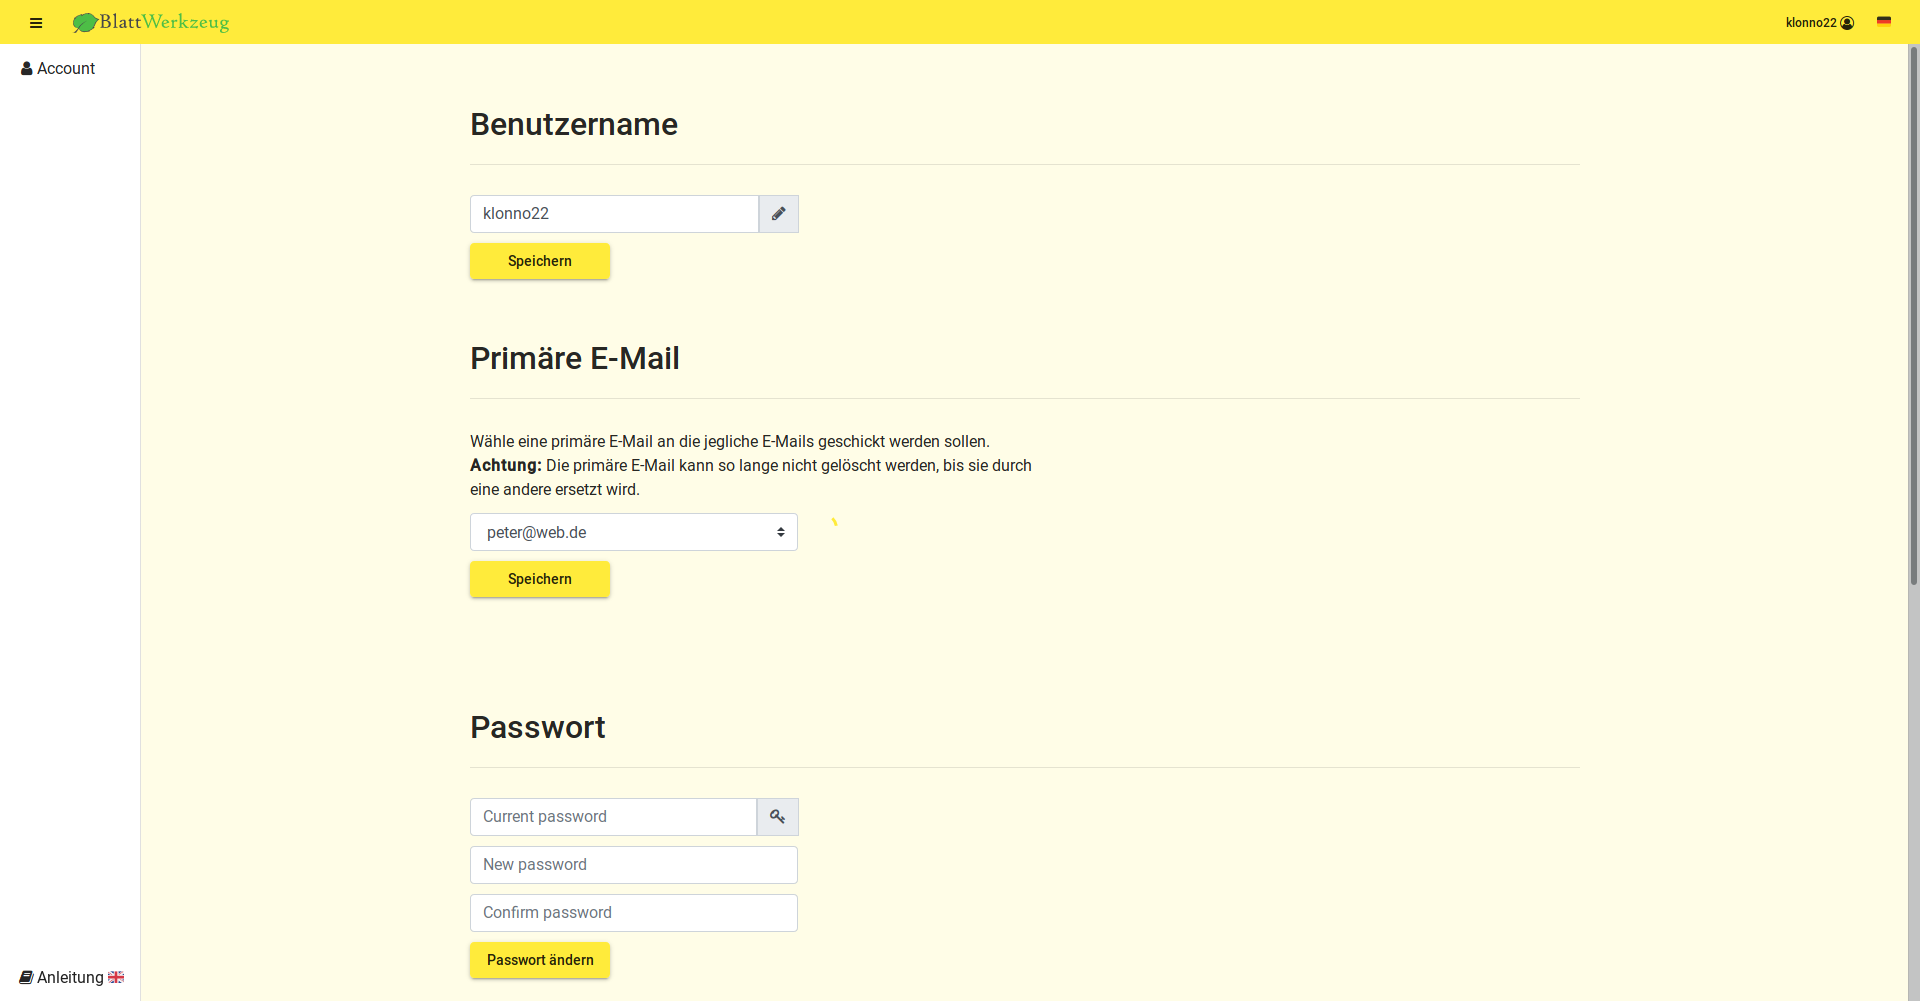
\includegraphics[width=\textwidth]{graphics/account-settings-1.png}
	\caption{Standart und erweiterte Ausführung eines validate-input}
	\label{fig:account_settings_1}
\end{figure}

\begin{figure}
	\centering
	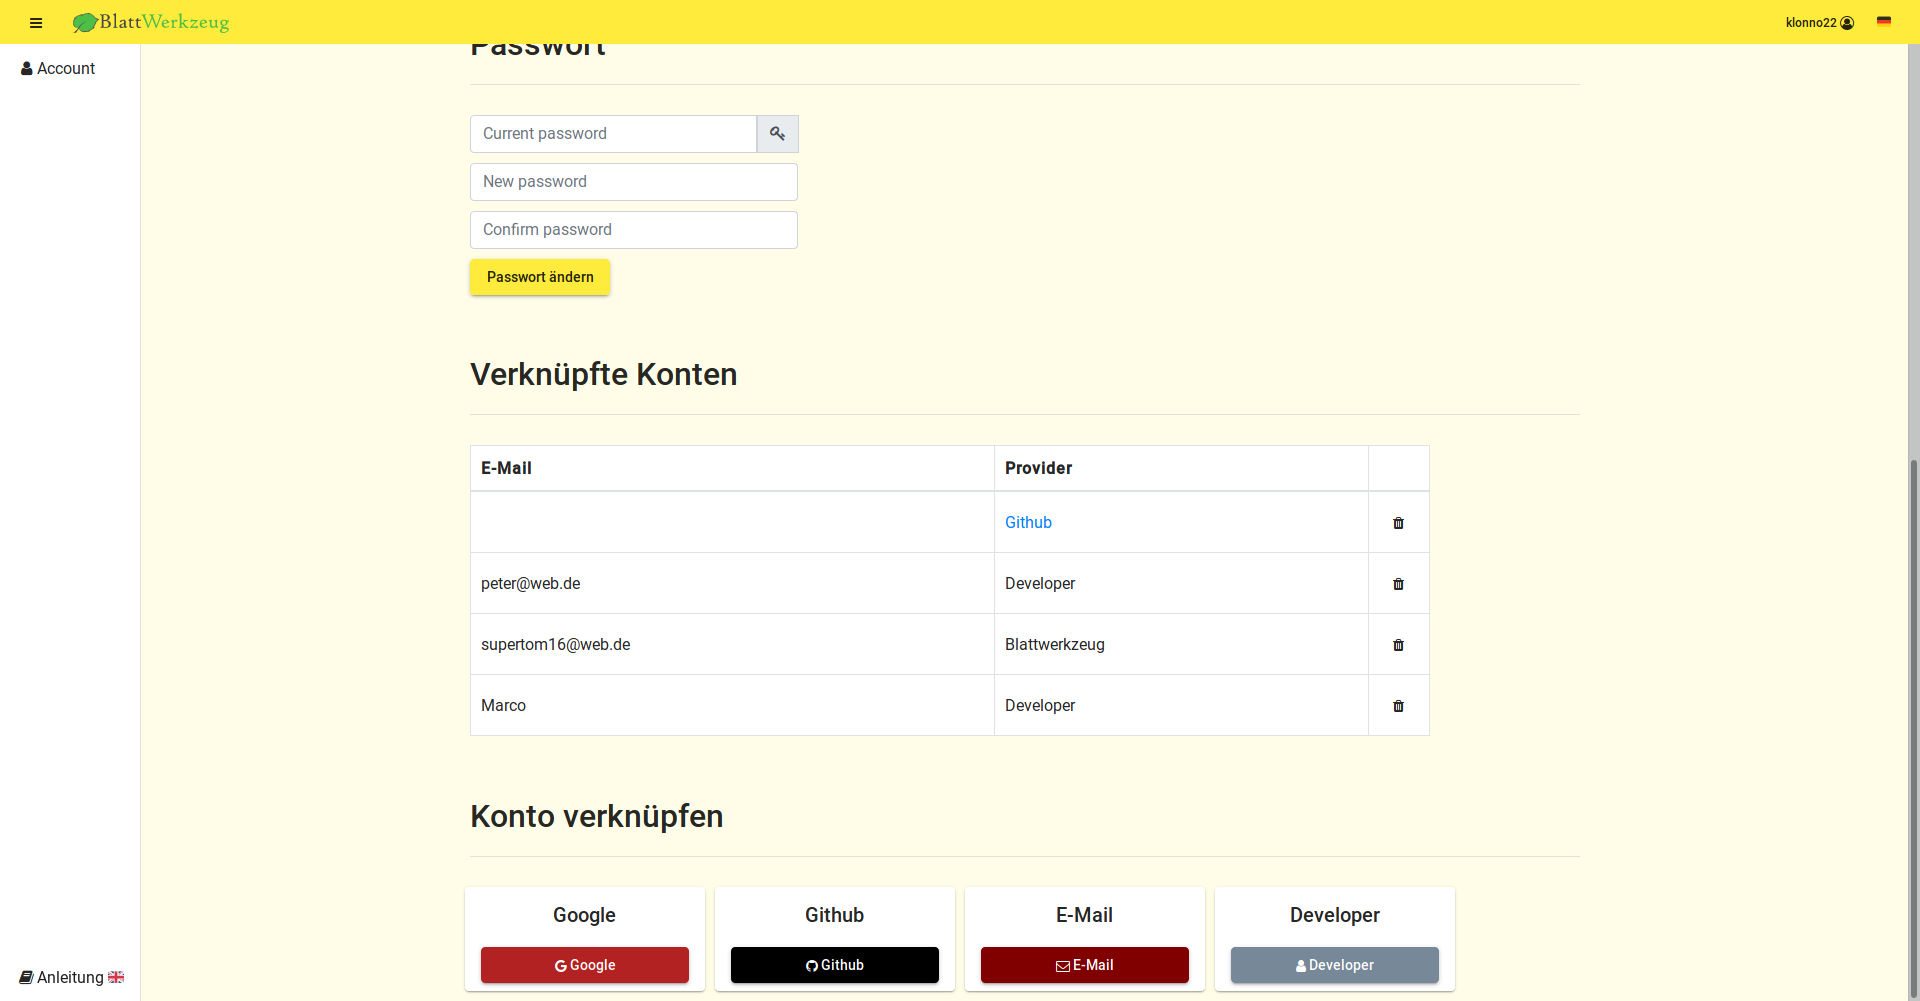
\includegraphics[width=\textwidth]{graphics/account-settings-2.png}
	\caption{Standart und erweiterte Ausführung eines validate-input}
	\label{fig:account_settings_2}
\end{figure}

\subsubsection{Wrapper-Komponenten}
\label{sec:client-wrapper-components}
Die Darstellung der Blattwerkzeug-Seite muss abhängig von den Rollen eines Benutzers sein. Hierfür ist es möglich die Unterteilung der einzelnen Codeabschnitte jeweils mit der Angular internen *If Direktive zu lösen. Eine weitere Möglichkeit wäre, die zu den Rollen angepassten Codeabschnitte jeweils in eigene Komponenten auszulagern. Ebenso ist es Möglich eine Wrapper-Komponente zu entwickeln, die dynamisch den Inhalt ihres Templates lädt und hierbei bedingt zwischen dem übermittelten Inhalt unterscheiden kann.

Das Nutzen der *If Direktive Angulars für jegliche Codeabschnitte, hat den Nachteil, dass erhöhte Coderedundanz vorkommt. Jede Komponente die Codeabschnitte abhängig von einer Rolle besitzt, müsste auf die jeweiligen Rollen eines Benuzers Zugriff haben. Dafür müsste in jede Komponente ein Service mit eingebunden werden, der die derzeitigen Rollen eines Benutzers an die Komponente ausliefert.

Die Unterteilung der einzelnen Codeabschnitte in eigene Komponenten hat den Nachteil das diese nicht flexibel sind. Eigene Komponenten würden sich stark auf die benötigte Rolle fokusieren. Sollte der Name dieser Rolle geändert werden, müsste nicht nur die Rollen-Abfrage verändert werden, sondern zusätzlich der jeweilige Name der Komponente.

Eine Wrapper-Komponente die dynamisch ihren Inhalt lädt und gleichzeitig bedingt auf den Inhalt achtet, verhindert erhöhte Coderedundanz und ermöglicht eine einfache Erweiterbarkeit oder Veränderung der Komponente. Aus diesen Gründen wurde sich für diese Methode entschieden.
\begin{description}
	\item[may\_perform]\hfill\\
	Bedienelemente die von der jeweiligen Benuterrolle abhängen, wie beispielsweise der Speichern-Knopf eines Projektes, werden mittels may\_perform Wrapper-Komponente überprüft und dargestellt. Damit eine Überprüfung serverseitig stattfinden kann, wurde sich vorerst mit den zu übermittelnden Daten beschäftigt.
	eine Anfrage an den Server gestellt (Sektion \ref{sec:server-authorisation}).


	\item[is-logged-in]\hfill\\
\end{description}

\subsubsection{Routing-Guards}
\label{sec:routing-guards}

\begin{description}
	\item[MasterGuard]\hfill\\
	\item[AdminGuard]\hfill\\
	\item[LoggedInGuard]\hfill\\
\end{description}

%%% Local Variables:
%%% mode: latex
%%% TeX-master: "Tom - Thesis"
%%% End:
